\documentclass[11pt]{article}
\usepackage[small,compact]{titlesec}
\usepackage[margin=0.25in]{geometry}
\usepackage{subcaption}
\usepackage{common}
\title{\begin{center}
{\Large Practical 3: Preferences in Streaming Music}
\end{center}}
\author{ Baojia Tong (baojia.tong@cern.ch)\\Yuliya Dovzhenko (dovzhenko@g.harvard.edu)\\Alan Legoallec (alanlegoallec@g.harvard.edu )\\\\Public Repository: https://github.com/tongbaojia/pubcs181}
\begin{document}
\maketitle{}
\section{Data}
\subsection{Additional Features}

\subsection{Data Preprocessing for Singular Value Decomposition}
In order to perform matrix operations on our data, we had to translate it from dictionary form to a sparse matrix. We used lil\_matrix format from scipy.sparse, because it is intended for incremental construction of the matrix, one value at a time. We then called the singular value decomposition function intended for sparse matrices. We constructed our predictions in lil\_matrix format as well. With these 

To avoid unrealistic features in the data, we first  filled in missing datapoints (the ones to be predicted) with median number of listens for the user. We then normalized each user's row to the total number of listens. We explored filling in with means, filling in with zeros, not normalizing, and normalizing to the median. We found the best performance when filling in with the median, and normalizing to the total number of listens. To undo the normalization after predictions have been made, we kept track of total listens for each user. 
 
To obtains plots in Figs. \ref{SVD_k}-\ref{SVD_g}, we selected 5\% of our data at random to use as a test set for cross-validation. 
\paragraph{} 
\section{Results}
\paragraph{} We explored four different methods and compared the results. Kaggle scores obtained by our methods are summarized in table \ref{tab:results}. 
  \begin{table}
\centering
\begin{tabular}{llr}
 \toprule
 Model &  & Acc. \\
 \midrule
 \textsc{Baseline} & &137.79146\\
 \bottomrule
\end{tabular}
\caption{\label{tab:results} Summary of our best prediction accuracies on the kaggle test dataset.}
\end{table}


\subsection{Singular Value Decomposition}
For this section, we read a high-level summary of the use SVD in the netflix competition\cite{SVD}, as well as the wikipedia page about singular value decomposition. 

Singular value decomposition is an approximate diagonalization procedure, applicable for non-square matrices. It yields approximate eigenvalues (singular values) and approximate left and right eigenvectors. We have to distinguish between left and right eigenvectors, because they represent distinct things and have different dimensions. 

\begin{equation}
X = USV
\end{equation}
Here $X$ is the matrix whose rows represent users and whose columns represent artists. Rows of matrix $V$ are orthonormal eigenvectors in the artist space, i.e. vectors in 2000-dimensional space corresponding to the directions of the largest variability in the data. Each user is then represented by a row of $V$, which contains weights asssociated with every eigenvector in $V$. Intuitively, each user is a weighted combination of several music ``trends'', where the trends are represented by vectors in $V$. A schematic representation of singular value decomposition is shown in Fig. \ref{SVD}.
\begin{figure}[] 
\centering
        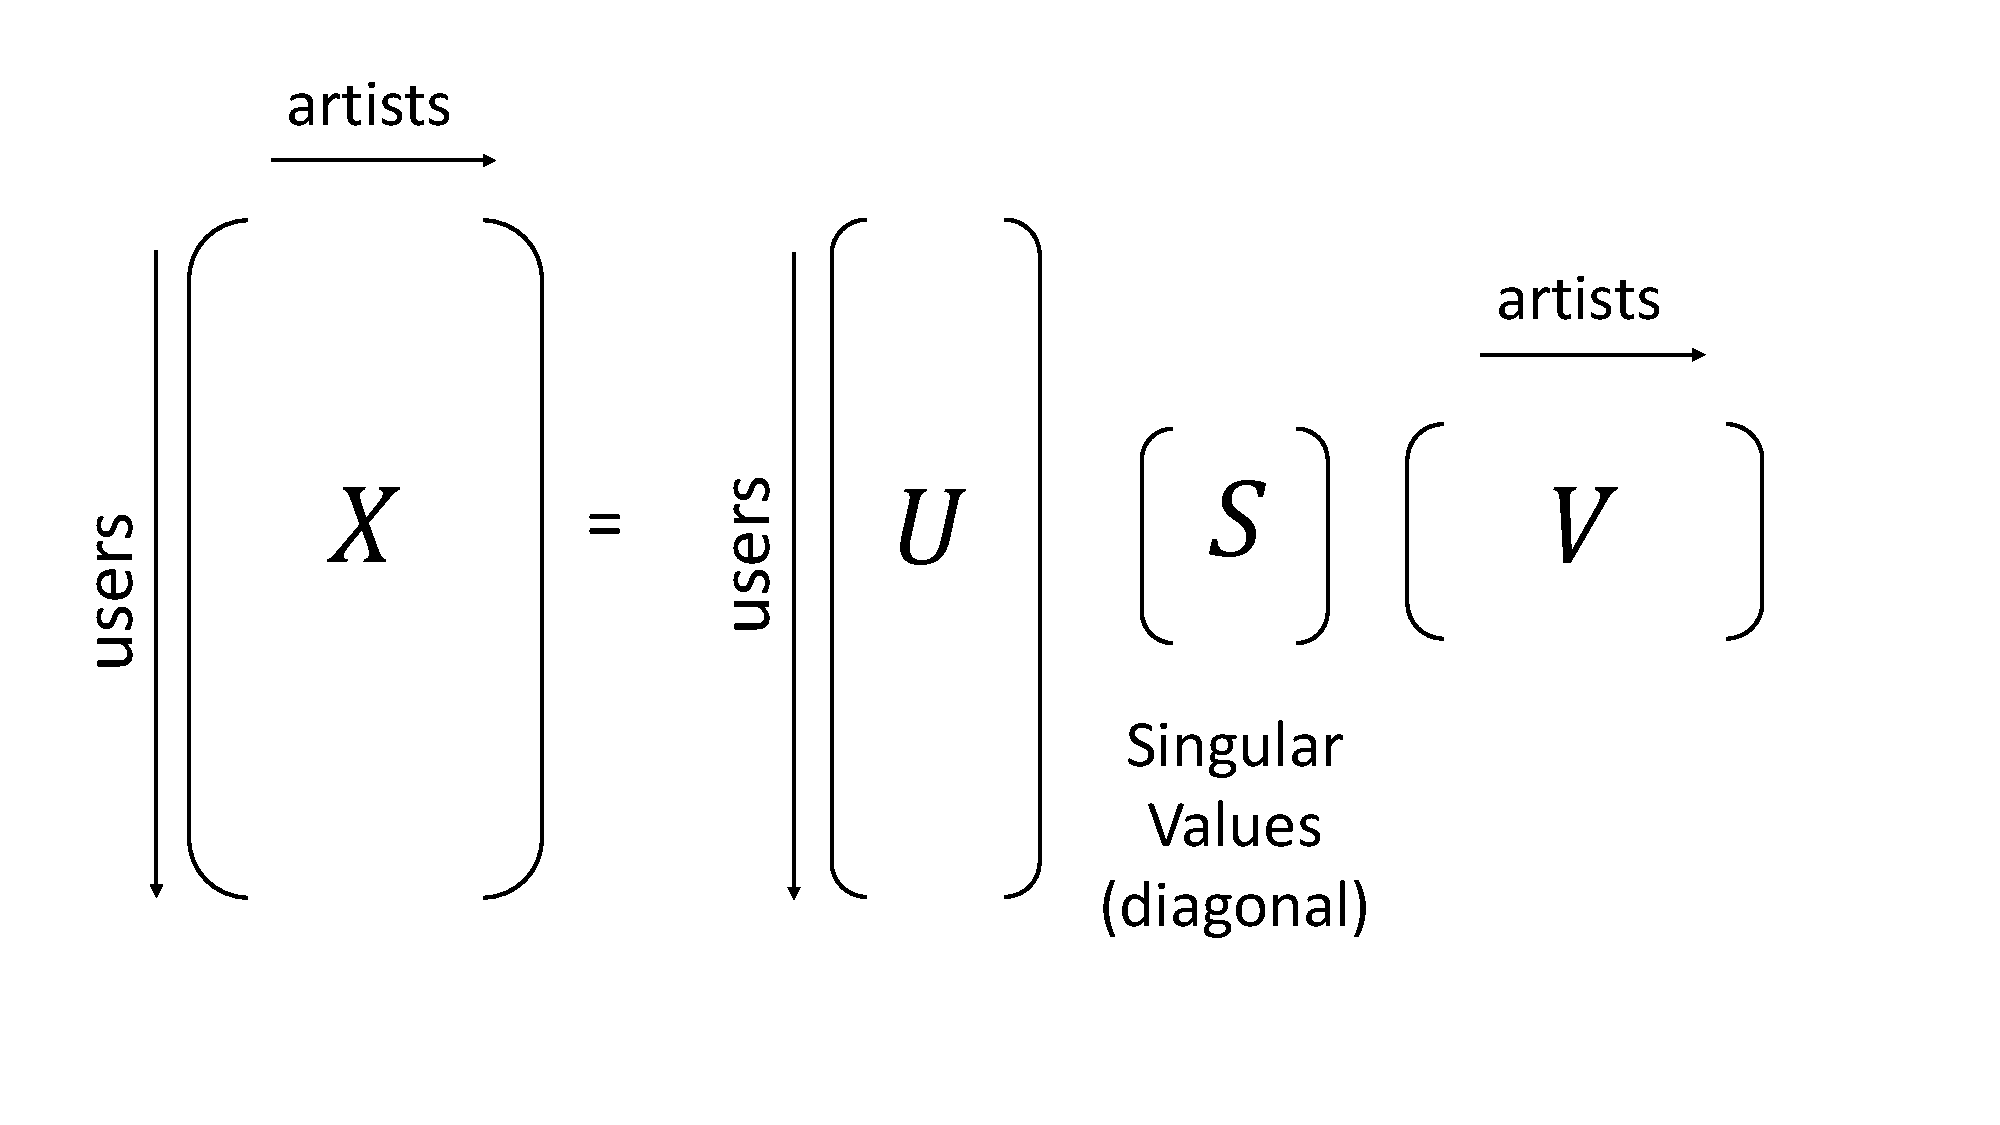
\includegraphics[width=0.6\textwidth]{Plots/SVD.pdf}
        \caption{Illustration of Singular Value Decomposition.}
            \label{fig:SVD}
\end{figure}

The number of singular values, $k$, is a parameter we pass to the SVD function. Once a diagonalization is obtained, there are many possible ways to proceed. Because of time constraints, we limited ourselves to two simple approaches:

\begin{enumerate}
\item First, we predict total number of listens of user $i$ to artist $j$ according to the following equation:

\begin{equation}
n_{ij} = U[i,:]SV[:,j]
\end{equation}
where $U[i,:]$ denotes $i$'th row of matrix $U$. We calculated mean error of the prediction as function of $k$, the number of singular values. Our results are plotted in Fig. \ref{SVD_k}.We saw the error in our prediction decrease steadily as function of the number of singular values, reaching below 160 with $k = 800$. While the trend was promising, we ran into memory constraints before we could beat the baseline. 

Another concern is that, with $k$ approaching half of the total number of artists, we may be in serious danger of overfitting, and in fact we are simply approaching the median values we initially used to fill in the missing values in the data. Intuitively, we would not expect to find as many trends as there are artists.

\item We attempted to improve on the basic SVD prediction by taking advantage of the reduced dimensionality of the data after decomposition to find $g$ nearest neighbors of a given user. We used  the KDTree library from the scipy.spatial module, which has efficient methods for finding a given number of closet vectors to a given vector. We used rows of $U$ to compute user-to-user distance. We then used an average of the number of listens to the same artist by nearest neighbors to predict listens of a given user. Mean error as function of $g$, the number of neighbors, is plotted in Fig. \ref{SVD_g}. The averaging was done after normalizing each user's number of listens. While the error decreased with group size, the computational cost rose very quickly, making it difficult to find convergence in the error.
\end{enumerate}


\begin{figure}[] 
\centering
    \begin{subfigure}[!t]{0.31\textwidth}
        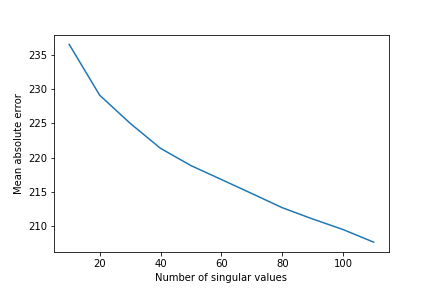
\includegraphics[width=\textwidth]{Plots/SVD_k_100.png}
    \end{subfigure}
        \begin{subfigure}[!t]{0.31\textwidth}
        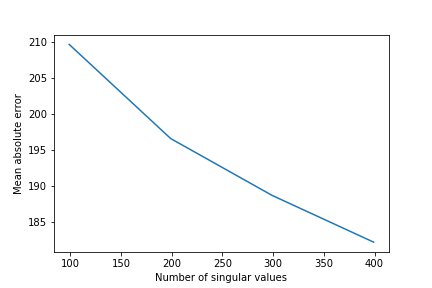
\includegraphics[width=\textwidth]{Plots/SVD_k_400.png}
    \end{subfigure}
            \begin{subfigure}[!t]{0.31\textwidth}
        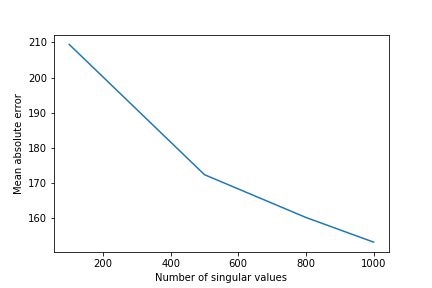
\includegraphics[width=\textwidth]{Plots/SVD_k_1000.png}
    \end{subfigure}\\
        \caption{Mean error as function of $k$, the number of singular values used in SVD. The error is monotonically decreasing.}
            \label{SVD_k}
\end{figure}


\begin{figure}[] 
\centering
        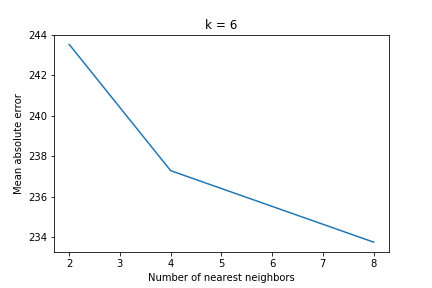
\includegraphics[width=0.31\textwidth]{Plots/SVD_group_8.png}
        \caption{Mean error with fixed $k=6$, and averaging number of listens from $g$ nearest neighbors in order to make a prediction. $g$, the number of neighbors, is plotted on the axis.}
            \label{SVD_g}
\end{figure}


\paragraph{}.
\subsection{Method 2}
\paragraph{}

\section{Discussion} 

User median is an unexpectedly good predictor, and was hard to beat.

We explored dimension reduction due to sparse nature of the data. We were expecting to find underlying patterns in the data, e.g. a certain subset of users liking a certain genre of music. We pursued SVD. We expected it to perform very well, because of its use in the Netflix prediction challenge. One notable difference is that all Netflix ratings are numbers between 1 and 5, while our number of listens vary considerably from user to user. 

A key difficulty of this project is incomplete data. If a certain user has not listened to an artist, that could mean that the user is not interested in the artist. It could also mean that the user would like the artist, but hasn't listened to him or her yet. It was probably for this reason that working with pure listen counts may have been the wrong approach.

 \begin{thebibliography}{1}

  \bibitem{SVD} Stephen Gower. {\em Netflix Prize and SVD}. http://buzzard.ups.edu/courses/2014spring/420projects/math420-UPS-spring-2014-gower-netflix-SVD.pdf (2014).

  \end{thebibliography}
\end{document}

